\documentclass[a4paper,12pt]{report}

\usepackage[utf8]{inputenc}
\usepackage[english]{babel}
\usepackage{natbib}
\usepackage[T1]{fontenc}
\usepackage{setspace}
\usepackage{graphicx}
\usepackage{hyperref}
\usepackage{csquotes}
\usepackage{subcaption}
\usepackage[top=3.5cm,left=2.5cm,right=2.5cm,bottom=3.5cm]{geometry} % 'showframe' to see borders

\graphicspath{ {images/} }

\def \reportTitle{Recommending photo filters via image content in a Web App \& REST API}

\title{\vspace{-2cm}
\includegraphics[width=5cm]{mmu-white.pdf}\\\vspace{4cm}\reportTitle\vspace{1cm}}

\author{Joshua Bridge\\14032908\\joshua.m.bridge@stu.mmu.ac.uk}

\begin{document}

\maketitle

\doublespacing

\begin{abstract}
  \textit{To be completed.}
\end{abstract}

\onehalfspacing
\tableofcontents
\doublespacing

\listoffigures

% \listoftables

\chapter{Introduction}
  % TODO Complete summary of introduction
  % ADD

  \newpage

  \section{Aims}
    In this report the following goals are what is expected to be achieved in the creation of the product:

    \begin{enumerate}
      \item To reduce complexity, information overload, and time spent for users when trying to customise photographs - usually in the expectation that the photographs will later be shared on social media.
      \item To create a secure platform for other applications to utilise the advancements made in this project.
    \end{enumerate}

  \section{Objectives} \label{sec:objectives}
    The objectives below describe in more detail a set of more specific goals which should be achieved in order to create a successful product:

    \begin{enumerate}
      \item \label{obj1}Implement a simple online web application for filtering images using a framework or library designed for front-end development across multiple platforms.
      \item \label{obj2}Implement a back-end application which is able to process images including applying filters and creating thumbnails.
      \item \label{obj3}Research various recommender systems to determine the common technologies/solutions for solving the problem of recommendations.
      \item \label{obj4}Implement a recommender system which is able to suggest photo filters to users based on image content.
      \item \label{obj5}Implement a RESTful API which exposes both the recommender system and the filtering system to the front-end web app and allows developers to connect them into their own applications.
    \end{enumerate}

  \section{Digital image processing}
   Image processing deals with the analysis and manipulation of image data. An example of image processing is the use of digital signal processing. This involves converting analog sensory data from a digital camera sensor into a computer-interpretable format with minimal data loss from external sources such as noise and distortion.\\

   \subsection{Bitmaps}
     Before you are able to analyse an image, you must first represent the data in a way that it can be interpreted by a computer, and a human. One basic form of doing this is via a bitmap image. A bitmap - as its name implies - is a simple spacial mapping of values (bits) along a horizontal axis (x) and vertical axis (y). Using a greyscale image as an example, a bitmap representation of this would contain a number of values (or ‘pixels’), the number of which is equal to the product of the sizes of the x and y axes. Therefore an image of size 200 x 200 would contain 40,000 pixels. Each of these pixels contains an integer value representing brightness, typically ranging from 0 - 255 (the total value range of an 8-bit integer), ‘0’ being completely black, ‘255’ being completely white.

     A colour image follows a very similar format, except now each pixel contains three brightness values instead of one. Each of these values map to the brightness of the colours (or ‘channels’) red, green and blue - in that order. Therefore a pixel with values (0,255,0) would be entirely green and a pixel with values (0,0,255) would be entirely blue. It should be noted that when these colours are displayed on a computer screen their colour values are additive (i.e. they can mix together to form a different, brighter colour). A pixel with values (0,255,255) would therefore represent cyan, and finally a pixel with values (255,255,255) would represent white.

   \subsection{Image processing tasks}
     There are several methods of improving the results of image analysis, one of which is to run an image processing algorithm against it. Generally this is to make the image clearer by sharpening it or removing noise - these are often referred to as low-level processing methods \citep{sonka2014image}. While these methods are often applied to make analysis by a computer a lot easier, they also can be used to increase the ‘clarity’ or the percieved ‘beauty’ of an image when viewed by a human.

     \subsubsection{Sharpening}
       For an image to be captured, it must first enter through some kind of lens which refracts the incoming light into a ‘focal point’ onto which some kind of light-sensitive surface is placed such as a digital image sensor. In order for an object to be perfectly ‘in focus’ it must be at the optimal distance from the lens - an area known as the ‘focal plane’. If the subject of a photograph is not near enough to the focal plane (either in front of it or behind it) then the subject will appear to blur.

  \section{Computer vision}
   Computer vision involves modelling the human vision system in such a way that a computer can interpret abstract visual data.

\chapter{Literature Review}
  In order to understand the background of the technology involved in this project, it is necessary to complete a significant review into the current and past literature. This will help form a basis of knowledge from which the future development and analysis of the proposed system will utilise and build upon. This research will be vital in order to make use of the most optimal technology for any given problem.

  The following review will be an investigation into the current knowledge of the major components of the proposed system, which are as follows:

  \begin{itemize}
    \item The recommendation system.
    \item The image filtering system.
    % \item The web-based user interface.
  \end{itemize}

  \section{Recommendation systems} \label{sec:lit-recc}
    As defined in \cite{ricci2011introduction}, recommending content is a problem which involves attempting to predict what a user may desire at any given time when using a system. In the ‘internet era’ applications of this are far-reaching, such as recommending products on Amazon.com \cite{linden2003amazon}. Recommendation systems are a popular topic due to the \textquote{abundance of practical applications that help users to deal with information overload and provide personalized recommendations, content, and services to them} \citep{adomavicius2005toward}.

    \cite{jannach2010recommender} describe three different methods for giving recommendations: Collaborative, Collaborative, Content-based, and Hybrid.

    \subsection{Collaborative recommendation}
      When using an online streaming platform that serves video content such as Netflix or YouTube, a user will visit their site looking for something to watch. The problem faced by these sites is trying to find content that the user hasn't seen before, but will align with the user's interests enough to make them want to watch it \citep{davidson2010youtube}, \citep{gomez2016netflix}.
      The information needed to carry out such a prediction can include the semantic value of the entire users history of interaction with the system (often referred to as \textit{metadata} \citep{duval2002metadata}), from which preference can be extrapolated. If there is not enough metadata about the user from which to extrapolate preference with reasonable certainty, then preference can be inferred from other users of the system - especially users with a similar predicted preference.

    \subsection{Content-based recommendation}
      There can sometimes be barriers to using collaborative recommendation, such as when the ‘cold-start problem’ is present. This problem describes when a user has just signed up to a website, it will not yet have enough information / user history to recommend them content \citep{schein2002methods}.
      In this situation content-based recommendation could be used more effectively to build up more reliable recommendations \citep{lops2011content}.
      There are different kinds of content-based recommendation, as it can be applied to many different kinds of content. For example a system may work differently if the content is user-generated as opposed to internally or computer generated, where the information would likely be provided already. In a system with user-generated content, the information about that content would have to be inferred, or provided by the user.

      \subsubsection{Feature extraction for content analysis}
        When content is user-generated and without a definition provided alongside it, its definition must be derived. For textual data this can be done by analysing the words and extrapolating a commonality between keywords to find a prevailing subject \citep{sanderson1999deriving}.
        This type of process is often referred to as ‘Feature extraction’ \citep{guyon2006introduction}.
        When analysing raw data such as an image file or an audio file, this becomes a much more difficult task as you must first find a way of deciphering the content before deriving the subject or meaning.

        Deep learning has recently become a common way of deciphering this content, including for image, audio, and video content types \citep{coates2011analysis,ciregan2012multi,lee2009unsupervised,mobahi2009deep}.
        Spotify has implemented this kind of deep learning to determine genre types from raw audio data - see section \ref{discoverweekly}.
        This can be applied to image data also, for example in the context of a search algorithm, it would bring the most relevant images by content to the top of the results \citep{yee2003faceted}. This works similarly to how a recommender system will select the most relevant items for the user to see.

        Google's neural network implementation has proven to be a very reliable system for image classification \citep{krizhevsky2012imagenet}.
        As it has a very high accuracy on most image types, it would be reasonably effective for providing a basis of feature extraction for use in a recommender system. In the system proposed in this report, scene classification along with prevailing colours in the image would be an ideal input into the recommendation system for determining optimal image filters.

    \subsection{Hybrid recommendation}
      Generally, hybrid recommendation applies both of the previous methods together in order to draw up a more comprehensive list of recommendations, in order to avoid the individual weaknesses of both types.

      \subsubsection{Spotify - Discover Weekly}
      \label{discoverweekly}
        Discover Weekly is a playlist made every week for every user of Spotify. Instead of getting humans to curate a playlist for each and every user, an algorithm is used to try and find a set of songs which it predicts the user will like, but hasn't listened to before. As described by \cite{popper2015dw} it does this by mixing collaborative and content-based recommendation. The first is done by analysing all playlists on spotify and determining their similarity to playlists made by the user. The next step is looking for songs in those playlists that the user in question hasn't heard yet.

        \begin{figure}[ht]
          \centering
          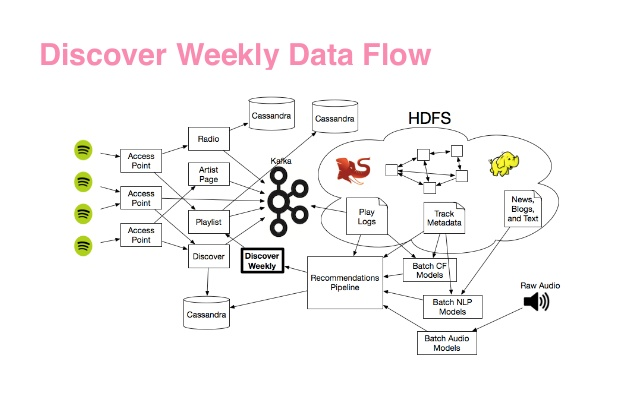
\includegraphics[width=\linewidth]{discoverweekly-dataflow}
          \caption[System component architecture of Spotify's ‘Discover Weekly’]{System component architecture of Spotify's ‘Discover Weekly’ \protect\citep{johnson2015dw}}
          \label{fig:discoverweekly-dataflow}
        \end{figure}

        The second, more complicated part of this process is the content-based recommendation. Spotify's algorithms actually analyse the music data in several different ways to determine a users ‘taste’. The first is by defining the genres a user listens to, which it does by scanning music blogs for what genre a certain piece of music is described as being. Using this as a search, spotify can then look for other music in that genre to recommend. The arguably more complicated part of this process is the auditory analysis of raw music data. As shown in figure \ref{fig:discoverweekly-dataflow} the raw audio is converted into ‘batch audio models’ where they can be used as a basis for recommendations.

  \section{Image filtering system}
    There is little to no research into the area of developing new photo filters, likely due to the fact that filters can be very subjective in terms of what effect they have on an image. Furthermore the relation of that effect to how many people choose that filter for a certain type of photograph would require a large data-set. However it is possible to determine the most common types of photographs posted online, which will guide the process of creating filter templates.

    \subsection{Instagram} \label{sec:lit-insta}
      In order to create image filters that users would want to apply to their photographs, an assessment must first be made about that the type of photos people tend to post online. ‘Instagram’ is a popular online photo-sharing platform that attracts over 700 million users \citep{instagram2017users}. An investigation by \cite{hu2014we} revealed that the types of photos posted on Instagram could be roughly categorised into eight types: \textquote{self-portraits, friends, activities, captioned photos (pictures with embedded text), food, gadgets, fashion, and pets}. The study clarifies that ‘self-portraits’ (or ‘selfies’) made up 24.2\% of the images posted, and ‘friends’ made up 22.4\%, totalling 46.6\% of the images analysed. From this it can be hypothesized that creating filters which are complimentary for skin-tones would be a contributing factor to success when developing image-filters.

      \cite{hu2014we} however did not study a wide proportion of the Instagram user-base, in fact they only closely studied 50 users, out of an initial 95,343 ‘unique seed users’, from a user-base of more than 150 million when the study was taken place. Furthermore the study only analyses pictures posted online, to Instagram, with public profiles, and from users which had \textquote{at least 30 friends, 30 followers, and had posted at least 60 photos}. The system proposed in this report would not be limited in terms of where the resulting image would be posted, and has no requirement that the image be posted to an online website (other than the system itself). Therefore the findings in the study should only be used as a loose guideline for popular image categories when defining image-filter styles.

    \subsection{Personalisation of image enhancement}
      There has been some work done on the mapping of image enhancement styles to personal taste, although the field appears to be still in early stages. Two studies in particular have heavily contributed to the development in this field. \cite{kang2010personalization} found that when given a set of images, participants would deviate into different styles when asked to choose between two options of enhancement (e.g. lighter or darker). Furthermore, many participants preferred their own enhancement when compared to an averaged enhancement, suggesting that personalised enhancements would be a valuable tool.

      Using the work done by \cite{kang2010personalization} as a basis, \cite{caicedo2011collaborative} developed a method of personalised image enhancement that focused on putting users into groups (or ‘clusters’) that had similar tastes within image enhancement. Therefore when attempting to apply personalised enhancement on a per-user basis, instead of determining a specific users preference from scratch, the user's preference would only have to be mapped to a pre-defined group. Using this method the authors suggest that personalisation of image enhancement could be scale-able to large amounts of users.

  \newpage

  \section{Conclusion}
    Posting images online is fast becoming one of the biggest trends in recent history, as evidenced by Instagram's user-base expanding to over 700 million users \citep{instagram2017users}. While not much public research seems to have been carried out into the reasons why users pick certain styles of image-filters before posting, it certainly appears viable to aid them in making that process easier.
    The findings of this review suggest that feature extraction could be a useful tool in developing recommendations for filters. This would be carried out in the form of image classification, most commonly to determine whether a person is present in a photograph which would thereby influence the algorithm's decision of what filters to recommend to the user for a certain image.

    The findings of this review also suggest (mostly from \cite{kang2010personalization,caicedo2011collaborative}) that the field of personalised image enhancements (or filters) is a relatively new field of study, therefore there is a lot of room for collecting new findings by extending upon previous works in a new implementation.

\chapter{Design}
  In this chapter a detailed description of the product design will be laid out, including explanations for each choice of technology and how it will enable the product to achieve its goal. The product can essentially be split up into two major components - a RESTful API \& a web-based front-end. Creating an API is an important factor in the implementation as it defines how the flow of the client application will work. As a result, technologies must be chosen which easily make use of this type of application-flow such as a framework which integrates well with AJAX calls - a common way of connecting to APIs. The front-end development is also a crucial part of the implementation as it acts as a testing interface for the API. If the API is not structured well then designing a front-end around it is much more difficult, meaning any future developers wishing to use it might be dissuaded by its complexity and end up choosing a different service. Developing both at the same time makes it much easier to see how clients will access the service, therefore making it much easier to remove any complexity it may contain while the service is still being built.

  \section{Requirements} \label{sec:requirements}
    The application proposed in this report would be best utilised on multiple platforms \& devices, as the service it would offer is platform-independent (i.e. all you need is an image file). For this reason the primary focus will be making an online web-app, which connects to a seperate REST \citep{fielding2000architectural} API which performs the main functions of the application, without the clutter of the front-end mixing in with it. This would also allow other apps and services to utilise this API and integrate it with other apps, such as on social media apps when sharing an image.

    When designing a user-facing website and an API, there are certain considerations that have to be met, such as data security and ease of use. The following features define what the final product should achieve:

    \begin{itemize}
      \item A web-based user interface.
      \item A user-history (metadata) tracking mechanism.
      \item A RESTful API which can be utilised by any application.
    \end{itemize}

    Following these features, these are some of the things that should be taken into consideration when implementing these features:

      \begin{itemize}
        \item The application \& API should be relatively scalable with user traffic.
        \item It should not store any more information about users than it has to.
        \item It should maintain a reasonable level of security to prevent user-data from being stolen.
        \item It should not store user images after the user has finished using the application.
      \end{itemize}

  \section{Application architecture proposal}
    Figure \ref{fig:application-diagram} shows the proposed architectural flow for the product being created using an example image from \cite{cat2013image}. It shows how an image is uploaded to Amazon S3 before being analysed, then the filtered previews are uploaded to S3 before the API response is generated.

    \begin{figure}[h]
      \centering
      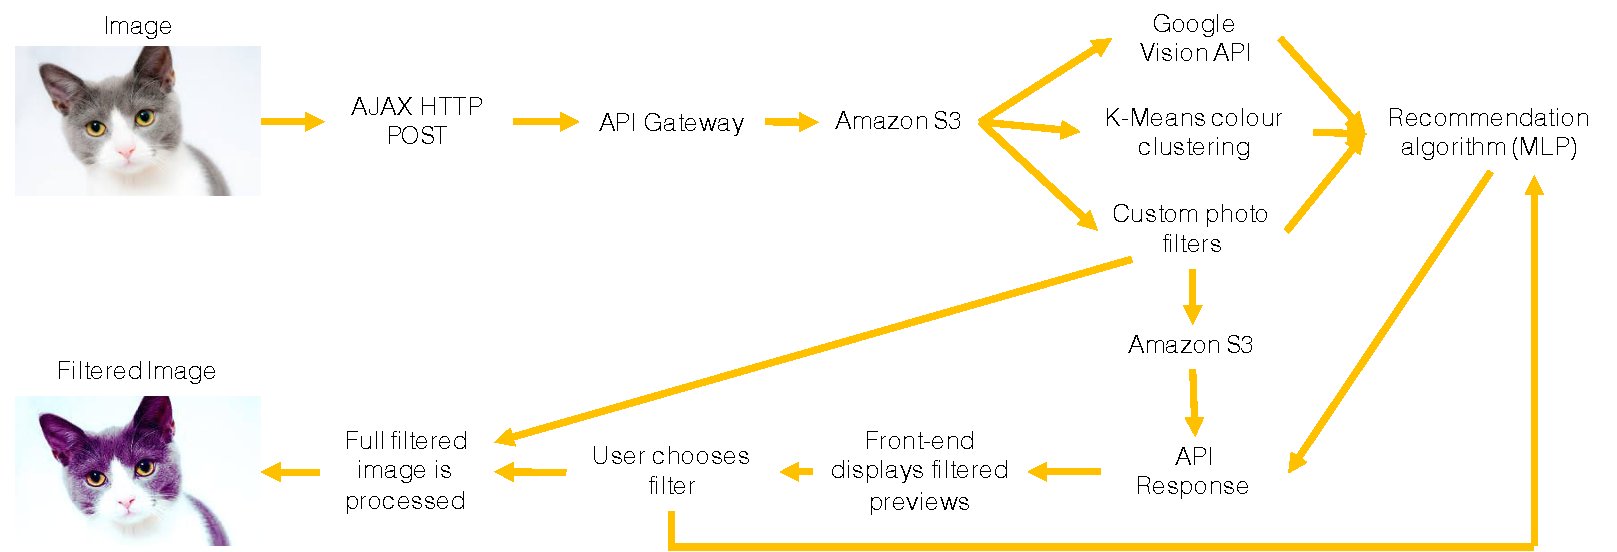
\includegraphics[width=\linewidth]{application-diagram}
      \caption{Architecture flow from client to API and their interactions}
      \label{fig:application-diagram}
    \end{figure}

    The final version of the API and front-end components will be hosted seperately on AWS due to its high configurability, with support for multiple different platforms and programming languages.

  \section{API}
    The API is to be written in Python (\url{https://www.python.org}) due to its high suitability for dealing with image data, web-access and recommender algorithms. The application is able to be completely self-contained as it can perform all of the functions required in a single project.

    \subsection{REST \& JSON}
      When developing an API, one of the biggest considerations which must be made is how the end user will be interacting with it. If an API is too complex and performs against a developers expectations, it could make it much more likely that developer might abandon it in favour of another competing product. Following an established architectural guideline makes it much easier to develop a clear API while spending more time focusing on developing core features. REST is a guideline developed by \cite{fielding2000architectural} which describes a resource-oriented method of designing APIs. This is the guideline that the API in this report will be attempting to follow.

      As many of the interactions with other services in this project are required to be completed using JSON as an interchange format, it stands to reason that it would be a good idea to also use this format for API responses. This is not just because it is popular, but also that converting data between different formats could be seen as unnecessary complexity within the application.

      \subsubsection{URI design}
        As there are not many operations which are required to be completed by the API, the number of endpoints can be kept to a relative minimum. Figure \ref{fig:api-call-flow} illustrates an example of how a client would connect to the API where the orange rows indicate a server action and the white rows indicate a client action.

        \begin{figure}[h]
          \centering
          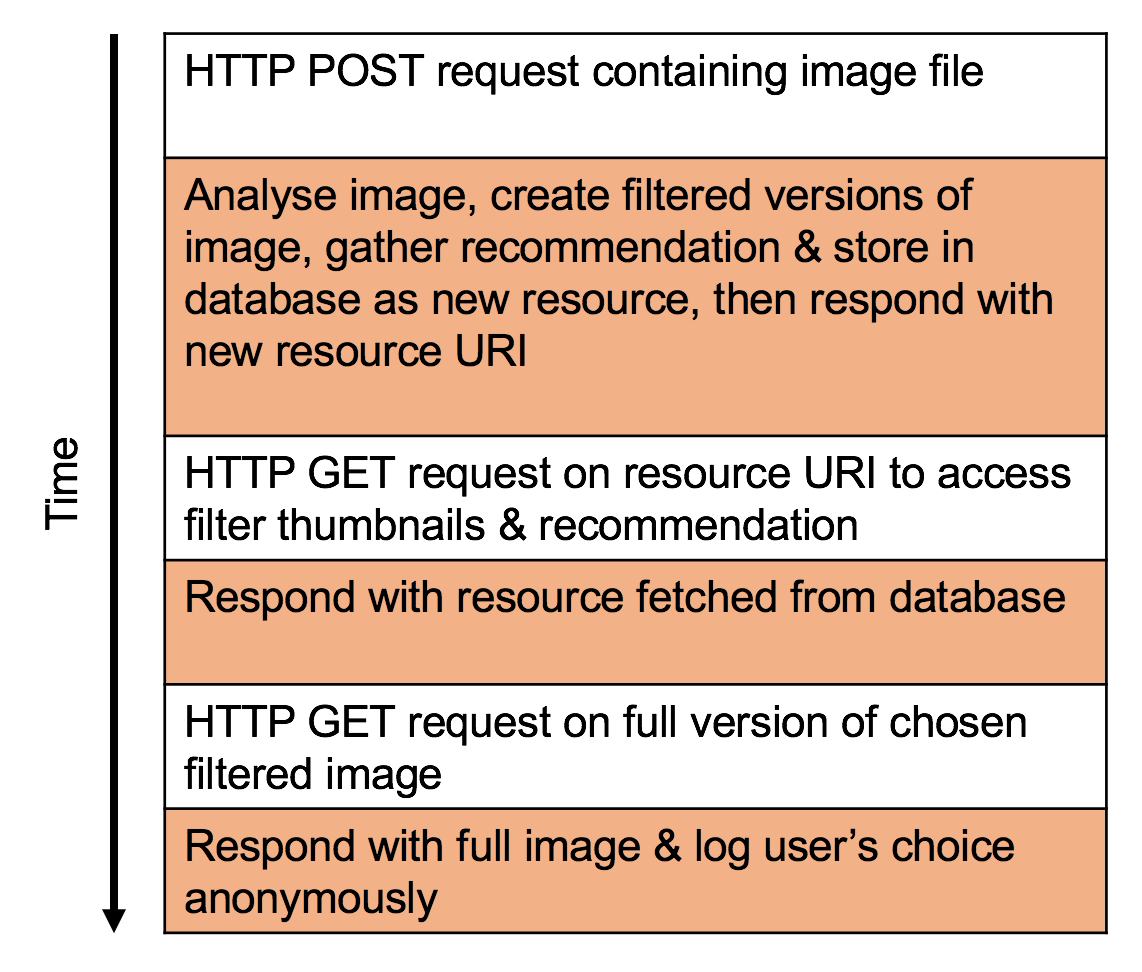
\includegraphics[width=0.5\linewidth]{api-call-flow}
          \caption{Example flow of API access from client}
          \label{fig:api-call-flow}
        \end{figure}

        Using figure \ref{fig:api-call-flow} as the expectation for what interactions will happen on the sever, a simple URI of ‘\texttt{/images/}’ can be created for the first HTTP POST request. Then the new resource URI in the accompanying response could be an extension of this, containing a generated unique id for the resource. For example ‘\texttt{/images/1234}’ can be used to access the resource. The full version of the image then can be available at ‘\texttt{/images/1234-filter-name.jpg}’, with that URI contained within the original resource body so the client can easily access it.

    \subsection{Web Framework}
      A simple framework for handling HTTP access to the API endpoints is critical when creating an application which is meant to be able to handle high-volume traffic. Flask (\url{http://flask.pocoo.org}) performs exactly this purpose as it is a very lightweight framework which provides very easy methods for transferring data in different formats such as JSON.

      Other frameworks could be considered for this purpose, however few match Flask in terms of low complexity and ease-of-use. Django (\url{https://www.djangoproject.com}) is another very common web framework for Python which comes with many useful features such as a built-in user system. Many of the features, however, are not required within this project and would only increase the complexity of the code in the application. When applying the Lean Software Develoment methodology \citep{poppendieck2003lean} this would come under the heading of eliminating waste - for example spending less time learning a complex framework and more time actually developing core features \& meeting requirements. Therefore Flask is a good foundation upon which to build a RESTful API that is easy to use \& easy to develop.

    \subsection{Database Storage} % mongodb
      A database is a crucial component within an application therefore choosing a suitable one is an important step in creating an application. The choice of database technology falls into a few categories such as SQL/NoSQL (or Relational/Non-Relational). There are several differences between these database types such as ability to scale and the types of data which can or should be stored by them. Non-relational databases are useful when the data to be stored is not of a strong structure, where relational databases are more suited for structured, related information. For example a relational database would be well suited for storing products on an online store, where different data such as products or orders can be stored in different tables, with connecting foreign keys. SQL databases are also very good at managing consistency e.g. when data is inserted into a table, there will definitely only be one entry input into the database. This is in comparison to NoSQL where horizontal scaling causes there to be a higher chance of duplicate entries, in an effort to ensure no data is lost while maintaining fast transaction speeds.

      NoSQL databases are often easier to host than SQL databases due to their ability to scale horizontally \citep{cattell2011scalable} rather than just vertically (i.e. adding more servers to handle load rather than upgrading from one machine to another higher power machine). This is applicable in the context of this project as a requirement (see section \ref{sec:requirements}) is that the application should be able to scale well with more users.

      When considering the type of data which needed to be stored by the application a NoSQL database seems to be best due to the non-relational types of data to be stored such as API responses. Furthermore speed is a key part as every bit of processing has to be done fast enough for the client not to time out waiting for a response. MongoDB (\url{https://www.mongodb.com}) is a popular NoSQL database with easy connectivity to python using the library pymongo (\url{https://api.mongodb.com/python/current/}). MongoDB is very fast with access speeds of up to 10 times faster than MySQL \citep{han2011survey} and also comes with a strong query language therefore it is highly suited for use in the application.

    \subsection{Image Filtering}
      The main bulk of processing done in the API can be broken down into three main components which are filtering, analysis, and recommendation. Filtering is the first step and will involve work to create multiple different photo filters which can be applied to any image which gets submitted to the API. Due to pythons ability to manipulate image data well using several different libraries such as NumPy (see section \ref{sec:numpy}) and Pillow (see section \ref{sec:pillow}).

      When an image enters processing it can be loaded into python using Pillow which creates an array containing each pixel value within the image. The pillow library provides many default methods for manipulating images such as changing brightness or contrast. Furthermore it contains methods which allow it to be transferred to different datatypes such as a NumPy array, where other kinds of mathematical operations can be applied to the pixel data such as linear interpolation. The image can also then be split into three different arrays with one for each colour channel of red, green, \& blue and then operations can be applied individually to create a colour effect on the image. For example if the red channel only was brightned by increasing each pixel value by a certain amount, then when the channels were put into a single image again this would give the image a red tint, which could be desirable for use as a filter.

      Due to the nature of the application trying to recommend filters, it would stand to reason that the filters in the application should be easily distinguishable to ensure maximum seperability between them. When being entered to the AI component (see section \ref{sec:mlp}) it is much better to have high seperability between classes (or filters) in order to find the relationship between input data and its classification.

    \subsection{Image Analysis}
      The second stage of processing (though not related to the first stage) is to analyse the image in order to gather input information for the recommendation algorithm. Providing raw pixel data would not be ideal when processing larger images as this will likely increase processing time greatly. When trying to build a dataset for use in training the recommendation algorithm it would not be ideal to store every picture input into the application as this violates one of the requirements in section \ref{sec:requirements}. Furthermore the raw pixel data will not provide extracted meaningful information such as dominant colours and face detection. Therefore, the best way to proceed is to extract and store information about the image itself without storing any actual image content. As found in section \ref{sec:lit-insta} self-portraits are a highly common type of image posted online so it could be meaningful to extract whether an image contains one or more faces in it. This information could affect how someone chooses which filter they would like to apply to an image so it is vital in this application to include this information. A link between a person in a photograph and the filter being chosen could exist if one of the filters was more complimenting to skin tones for example. In order to find the dominant colours in the image and apply face detection two different methods will be applied and are described below.

      \subsubsection{Dominant colours: K-Means} \label{sec:kmeans}
        K-Means clustering \citep{macqueen1967some} is a form of machine learning which performs a mathematical analysis on un-labeled data in order to find common groupings within that data. The number of clusters (or groupings) is first specified and the algorithm then splits the data points into that number of groups and then finds an average value for each cluster. K-Means has been used for image segmentation \citep{coleman1979image,shi2000normalized} which is an important part of computer vision. In this case K-Means clustering will be used to find the dominant colours within the image along with their amount of use within the image as a percentage. The colours found from this process will likely not be exactly as they appear in the image due to the averaging of each colour cluster to find the most common groups of colours.

        The K-Means algorithm used in this application will not need to be implemented as there is one provided by the scikit-learn library (\url{http://scikit-learn.org/stable/}) which meets all requirements and makes it easier to implement K-Means directly into the application.

      \subsubsection{Face detection: Google Vision API} \label{sec:visionapi}
        The Google Vision API (\url{https://cloud.google.com/vision/}) is a useful tool for performing a variety of image analysis steps such as face detection and logo detection. It can be accessed via a REST API using JSON as the request language therefore it should integrate into the application with relative ease using the libraries available in python such as ‘requests’ (\url{http://docs.python-requests.org/en/master/}). Google has not published what technology exactly powers the vision API other than saying in a blog post that it is run using machine learning and TensorFlow (\url{https://www.tensorflow.org}) \citep{vision2015blog}. However, due to the complex nature of face and logo detection it can be assumed that the systems behind the API are running some very complex machine learning models which require a lot of processing power to run. With this in mind it will be much simpler to integrate this API into the application rather than try to implement a custom version of face detection into the application.

    \subsection{Recommendation}
      The final stage of processing within the application is to get the recommendation for which filter would be best applied to the image.
      As discovered in section \ref{sec:lit-recc} a good way of doing this is to use neural networks in order to build a relationship between input data and a possible classification. Within this application a form of hybrid recommendation will be used whereby the input to the algorithm will be the results from image analysis as discussed in the previous section. In order to find a relationship between this data and a filter, some data will have to be provided by some initial prototype users in which they will choose a filter for a set of photos of their own choosing.

      Using the stored image analysis data as parameters and the chosen filters as classifiers, a machine learning model can be built which hopefully finds a significant link between image content and the filters which could get applied to them. This is a form of hybrid recommendation as the users interests are powering the recommendation but that information is linked directly to the content of the image, thereby mixing collaborative and content-based recommendation. However, this is not strictly including true collaborative recommendation as the users are not being recommended based on tastes of similar users, but more that the collective users are helping to power the content-based recommendation.

      \subsubsection{Multi-Layer Perceptron} \label{sec:mlp}
        Multi-layer Perceptrons \citep{minsky2017perceptrons} are a type of neural network which can be used for classifying non-linearly separable data. A multi-layer perceptron consists of 1 input layer, 1 output layer and 1-to-many hidden layers which contain neurons that perform an activation function on their inputs. In the case of this application the multi-layer perceptron will be used as a recommendation algorithm by ‘learning’ the connection between image content and image filters. While it may not be best suited for recommendation in place of deep learning for example (section \ref{sec:lit-recc}), the MLP is already implemented in scikit-learn (\url{http://scikit-learn.org/stable/}) and therefore will be much easier to integrate within the application. Furthermore supervised deep-learning is more suited to dealing with pixel data, which this application aims to not keep therefore training a deep-learning model would be much more difficult.

  \section{Front-end}
    A front-end is an ideal way to create a testing interface for the API and is a good way to advertise to potential users of the API. Therefore one should be built which is capable of running on multiple platforms including mobile phones and desktops. This is so that it is accessible to as many people as possible, by removing as many impedences to accessing the application as possible. The most suitable way of achieving this would be to make the front-end a web-based service which could scale to various screen sizes, and thereby making the application accessible to all with no downloads required.

    \subsection{Frameworks \& Libraries} % React
      To achieve the best results in terms of aesthetics, functionality and work-effort, a front-end JavaScript framework is ideal for achieving the best results in the shortest time. Their pre-made code structures often eliminate a lot of the grunt work from creating reactive user interfaces from scratch, therefore they are an obvious choice.

      While there is little in the way of academic comparisons between JavaScript frameworks as told by \cite{graziotin2013making}, a subjective comparison can be made to find the most suitable framework for this application. Two commonly used libraries/frameworks are React and Angular which are discussed briefly below.

      \subsubsection{React Vs Angular}
        ReactJS (\url{https://reactjs.org}) is a JavaScript library for creating user interfaces which was created by Facebook (\url{https://www.facebook.com}). As it is entirely in JavaScript and introduces a component structure which updates when any data state changes, it is a simple way to add lots of functionality in a short time. AngularJS (\url{https://angularjs.org}) is another JavaScript library however it is not the recommended version of angular which is Angular 4 (\url{https://angular.io}) and is a framework rather than a library. Angular 4 uses typescript which could introduce complexity and the framework comes with a lot of baggage which brings a steeper learning curve as discussed by \cite{neuhaus_2017}.

      \subsubsection{Choosing React}
        ReactJS is the library which will be used in this application due to its flexibility and ease of use with a relatively small learning curve. React Native (\url{https://facebook.github.io/react-native/}) is a variant which can be used to run the JavaScript code as a native mobile app. This is commonly used to build mobile apps, and has been done by some such as Instagram (as stated on the React Native website). While React Native will not be used in this report, it is important to bear in mind the code would be the same, and that React in general is highly optimised for mobile development. Due to these factors React is highly suited for the requirements of this application, as long as the final product is able to easily scale between different browser sizes including desktop and mobile browsers.

  \section{Use Case \& Class diagram}

\chapter{Implementation} \label{cha:implement}
  In this chapter the implementation for the application proposed in this report will be explained. Both the API and the front-end will be developed concurrently to ensure that each of them are able to interact with each other in the easiest way possible. For example if any issues were found when accessing the API using the prototype front-end then they could easily be fixed by changing how the API returns its data.

  Once the code for both the front-end and API has been finished, the resulting applications will be deployed to AWS (\url{https://aws.amazon.com}) and put under the domains of ‘\url{http://inflex.co}’ and ‘\url{https://api.inflex.co}’. Some prototype versions will also be tested throughout for hosting on AWS to ensure the final deployment will be successful.

  \newpage
  \section{API}
    In this section the implementation details for the API including filtering, recommendation and web responding will be explained.

    \subsection{Image handling} \label{sec:numpy} \label{sec:pillow}
      While python was chosen for its suitability for image handling, there is not much guidance online for how to handle images in the context of trying to apply photo filters to them. In order to do this a more fundamental understanding of how photo filters worked was required. Essentially it was found that colour effects can be applied individually to each channel (the red, green, and blue channels) in order to adjust the colour palette for that image.

      In order to do this an image must first be loaded into memory, which it was found can be done using the Pillow library (\url{https://pillow.readthedocs.io/en/5.1.x/}). Figure \ref{fig:image-loading} shows the code required to import an image into memory from an external URL using the Requests library (\url{http://docs.python-requests.org/en/master/}). This is then stored as an ‘\texttt{Image}’ object for which there are various methods within the Pillow library for performing enhancements such as sharpening, brightness adjustment, and contrast adjustment (though these are not per-channel adjustments, rather they appied globally to every channel).

      \begin{figure}[h]
        \centering
        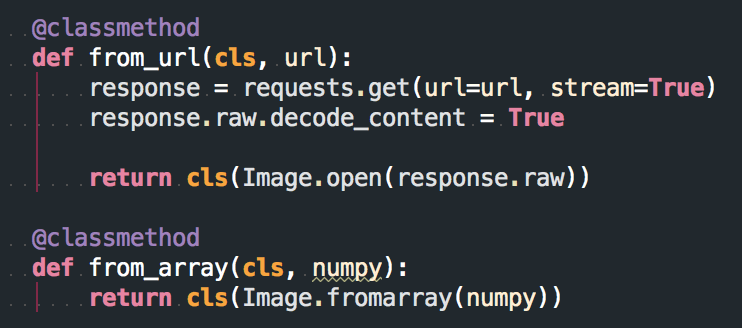
\includegraphics[width=0.5\linewidth]{image-loading}
        \caption{Loading an image into Pillow from an external URL, and from NumPy}
        \label{fig:image-loading}
      \end{figure}

      In order for per-channel adjustments to be made it was found that using NumPy (\url{http://www.numpy.org}) enabled much easier handling of pixel values, as they are treated as a multi-dimensional array with x and y dimensions along with an RGB value dimension. Note that most functions require the colour values to be in the range [0,1] as a floating point number rather than a [0,255] integer. The RGB dimension can be split into 3 different arrays for each channel and processed by increasing the channel values by a certain amount. Furthermore other operations can be completed such as adjusting the colour values using linear interpolation. Basically, this allows for fine tuning of colour values in that lower/darker values may get adjusted differently to higher/brighter values.

      In figure \ref{fig:filter-code} two of the filters which ended up being implemented are shown in the form of a python class. The classes extend an interface type class called ‘\texttt{BaseFilter}’ which contains the method stubs required of the filter. The ‘\texttt{apply()}’ method is the actual filtering method, which takes in another custom parameter called ‘\texttt{filterable}’. Most filters use the Pillow ‘\texttt{Image}’ object contained within that parameter and perform some contrast and brightness adjustments. The ‘Black and White’ filter uses only provided Pillow methods to convert the image into a black and white form of the image, as seen in figure \ref{fig:black-and-white-filter-code}. After the adjustments have been made, the seperate channels are then merged into a single array, where they can be converted back to a Pillow ‘\texttt{Image}’ object and returned as a ‘\texttt{Filterable}’ object for further processing.

      \begin{figure}[h]
        \centering
        \begin{subfigure}[b]{0.47\textwidth}
          \centering
          \caption{‘Joker’ filter class}
          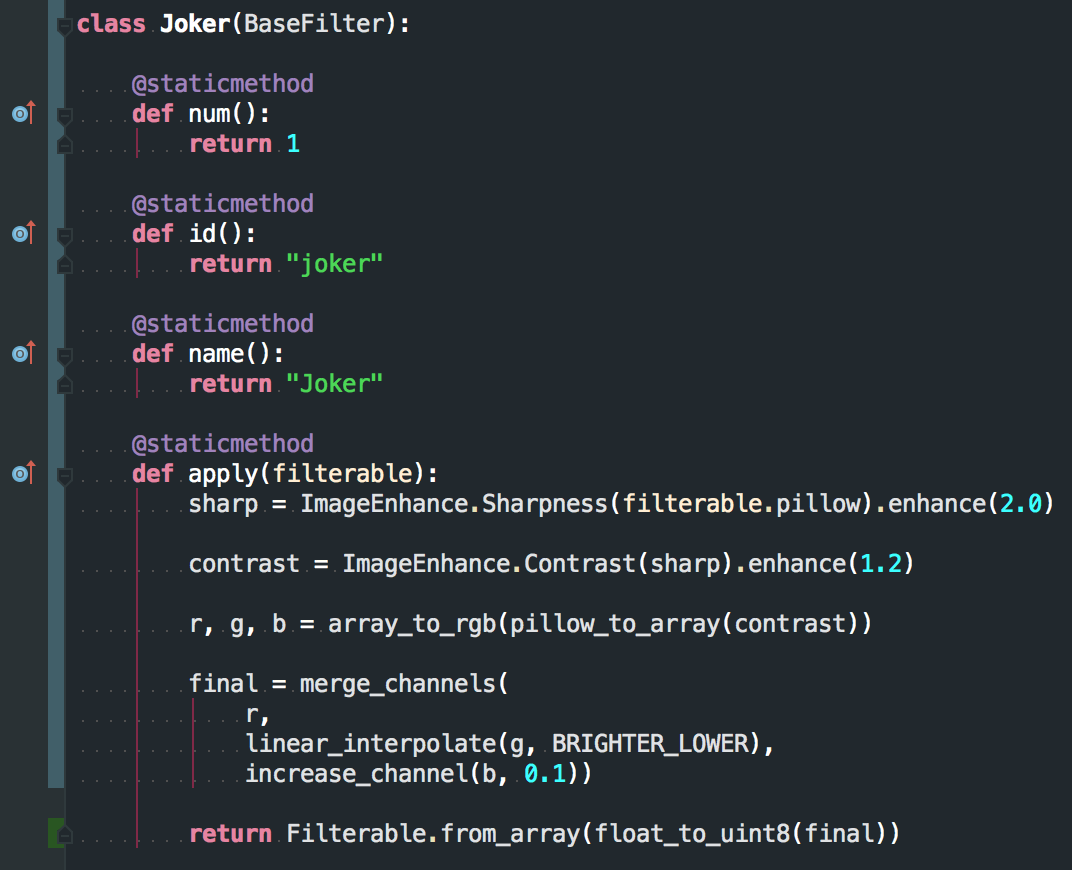
\includegraphics[width=\linewidth]{joker-filter-code}
          \label{fig:joker-filter-code}
        \end{subfigure}
        \begin{subfigure}[b]{0.47\textwidth}
          \centering
          \caption{‘Black and White’ filter class}
          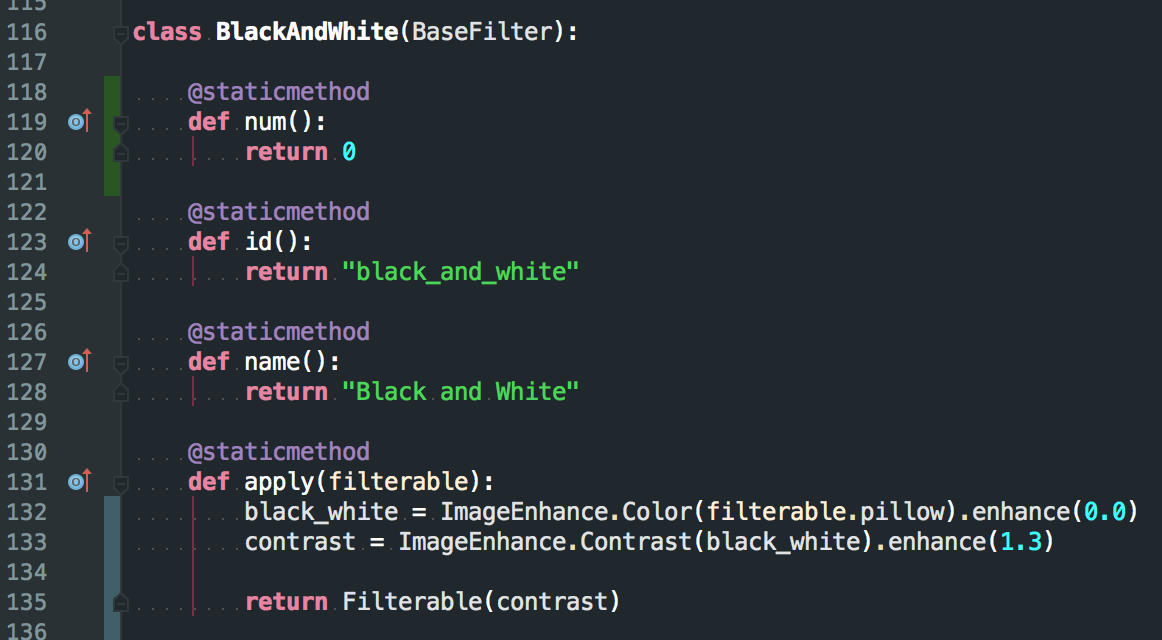
\includegraphics[width=\linewidth]{black-and-white-filter-code}
          \label{fig:black-and-white-filter-code}
        \end{subfigure}
        \caption{Python filter classes}
        \label{fig:filter-code}
      \end{figure}

    \subsection{Web Responding}
      Once the code had been implemented for adding filters to the images, the next step was to introduce a handler for HTTP API calls, where images can be uploaded to the application and then filtered using the aforementioned code. The Flask library was used to handle the HTTP requests by adding a python method for each URI address which needed to be accessed. It is quite easy to specify using Flask which HTTP method should be used for each URI and there are many built-in methods which handle file uploads to the server, along with restricting which file types can be uploaded. Figure \ref{fig:upload-api-method} shows how a URI structure can be defined using an annotation above a regular Python funtion.

      \begin{figure}[h]
        \centering
        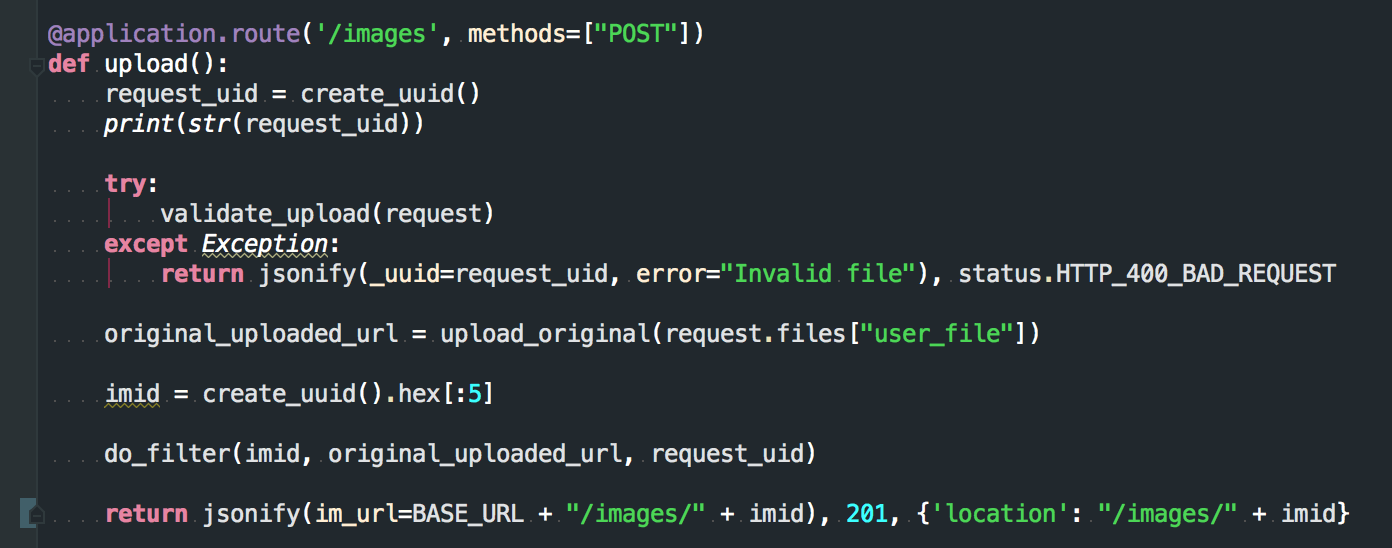
\includegraphics[width=0.7\linewidth]{upload-api-method}
        \caption{Flask image upload API method}
        \label{fig:upload-api-method}
      \end{figure}

      Due to Python being able to easily handle both image processing and web requests, it was relatively easy to link both of these functions together.  Once the URI routes had been set up all that was required to link them was creating a function which loops through each of the filter classes, passing in the original image each time. This was made possible due to the code design implemented in the previous section. As each filter was a subclass of ‘\texttt{BaseFilter}’, the built-in Python method ‘\texttt{\_\_subclasses\_\_()}’ returns any objects which are subclasses of that class. All that is then required is to loop through the returned list and run the ‘\texttt{apply()}’ method on each of them.

      Once the filters have been processed then it is possible to create thumbnails and previews of the resulting images using the methods on the ‘\texttt{Filterable}’ object mentioned previously. These thumbnails and previews will need to be uploaded somewhere in order to provide a link which a user can access to retrieve them. Amazon S3 (\url{https://aws.amazon.com/s3/}) was used as a remote hosting site due to its provided Python libraries which handle uploads to the service. For the images to be uploaded they must first be converted into a format such as a JPEG. To do this the built-in ‘\texttt{BytesIO}’ class was used along with the Pillow ‘\texttt{save()}’ method which writes the in-memory image array to a binary format.

      \begin{figure}[h]
        \centering
        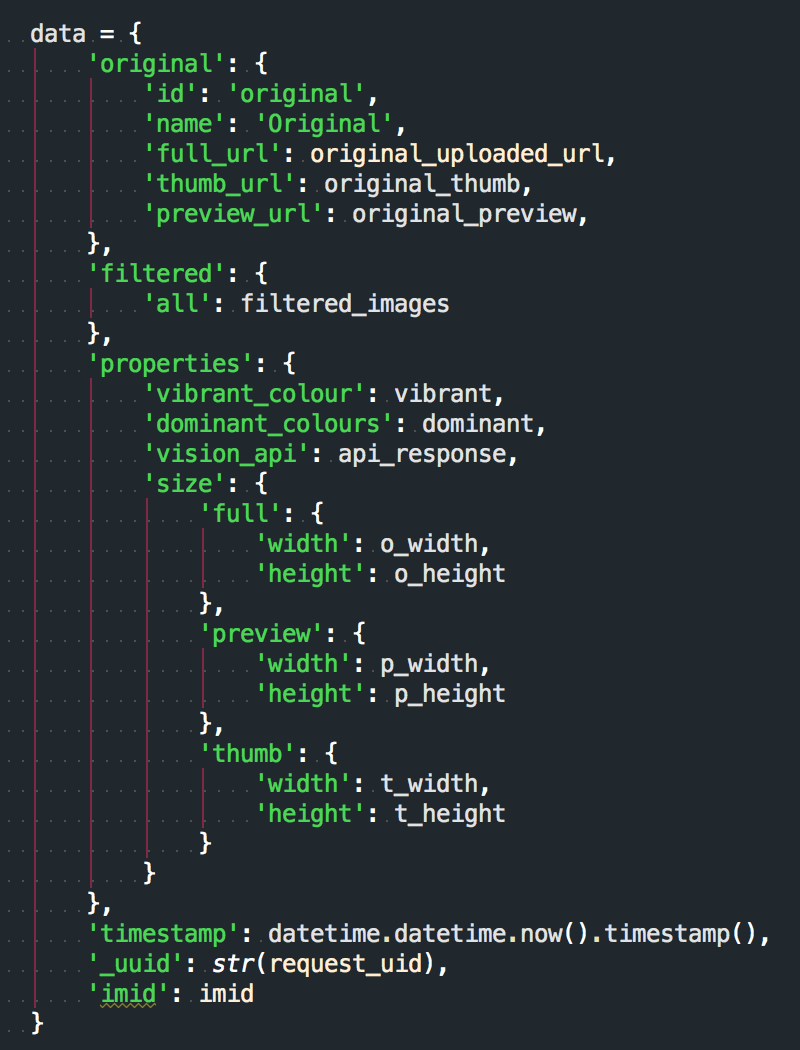
\includegraphics[width=0.4\linewidth]{python-json-dict}
        \caption{Python syntax for declaring a ‘\texttt{Dict}’ object}
        \label{fig:python-json-dict}
      \end{figure}

      Due to the syntax of Python it was very easy to define the JSON responses for each of the web methods. The Python ‘\texttt{Dict}’ object can be written in a very similar syntax to JSON and can be seen in figure \ref{fig:python-json-dict}. Further to this, the Flask library offers a JSON serializer method called ‘\texttt{jsonify()}’ which automatically converts its parameters into a JSON HTTP response.

      Finally, the REST constraints for the application were able to be met by using appropriate HTTP response codes for the API responses. An example of this is seen at the bottom of figure \ref{fig:upload-api-method} where the HTTP code ‘\texttt{201 CREATED}’ is returned along with the URL for the newly created resource.

    \subsection{Image Analysis}
      The two main methods for performing image analysis are using the Google Vision API and performing a K-Means colour clustering operation on the image to find the most prevailing colours within it. The K-Means algorithm is already implemented in scikit-learn therefore there was no need to implement it manually, which would have just introduced unnecessary work that goes against the ‘Eliminate waste’ principle of LSD \citep{poppendieck2003lean}.

      A value of 5 clusters was used in this instance of K-Means, which seemed to give a decent range of colours within the image without taking too much processing time. Also only a 100x100 sized version of the image is input into the algorithm to further ensure a fast enough response time for the API, at the risk of losing some colour detail. The algorithm requires a NumPy array, which was easy to supply by converting the Pillow image thumbnail to a NumPy array and re-shaping the array to the ideal shape of 2 dimensions.

      % TODO processing time

      After the K-Means analysis some further analysis is implemented on top of this in order to find the (subjectively) most vibrant colour out of the 5 colours found by K-Means. By using the HSV colour space (rather than RGB) which provides values of saturation and brightness it was easy to order the colours by the product of these two values, and then simply seleting the top item from the ordered list which gives arguably the most vibrant colour. This information could serve to be valuable for the recommendation algorithm as it could be possible to find a link between different vibrant colours and which filter a user chooses to apply.

      The next step of including a response from the Google Vision API is relatively simple. Using the API documentation by \cite{vision2018apidoc} as a guide, a request can be made in which an image URL is supplied along with the type of analysis to be conducted. Once again this request is made in JSON format which is easy to do in Python. In this case the ‘\texttt{FACE\_DETECTION}’ identifier is sent to the API and the response contains various information about any faces detected in the image. The detail from that response is not used however, as the only information which is desirable in this case is the number of faces in the image which can be found by adding up the number of objects in the ‘\texttt{faceAnnotations}’ array within the JSON response.

    \subsection{Recommendation} \label{sec:imp-recc}
      Using the data provided from the image analysis components described in the previous sections, the recommendation algorithm has been implemented with relative success. The Multi-Layer Perceptron is also implemented by scikit-learn therefore it made sense to use this implementation rather than create one manually. In order for the MLP to train itself on the data, the data needs to be in the form of a 2D array with normalised values along with a 1D array contiaining the corresponding classifications for each row in the first array. In order to provide such data a series of functions were implemented which convert the stored JSON data about the images (containing the image analysis results) into an array of raw values. More specifically, these raw values correspond to HSV colour values for the dominant colours, their proportional percentage values, and the number of faces in the image.

      The MLP is required to be trained manually by collecting all of the previous responses and formatting them in bulk to be supplied to the algorithm. With this in mind 10 users were asked to use a prototype version of the application and upload as many photos as possible, choosing the filter which they found most appropriate for each image while their choice was logged automatically, though completely anonymously. As a result of this 472 instances were then able to be used to train the MLP using a default train/test split of 75/25\% respectively. The structure used for the MLP was 3 hidden layers, each with 30 neurons, and a maximum training time of 1000 epochs.

      The results from the MLP were relatively poor, as the results after training multiple times appeared to differ greatly. Furthermore the average classification accuracy did not go above 40\% in any test. This could be due to a relatively low number of training instances, as well as the data having a poor link between input data and associated classifications.

      The trained model used in the system was selected due to its comparatively high average classification accuracy of 37\%, and was saved by serialising the MLP Python object using the Pickle library (\url{https://docs.python.org/3/library/pickle.html}). This model is then able to be loaded into memory when the application starts, in order to be used for classifying new instances supplied by the API code.

    \subsection{Database}
      The MongoDB database was used for a few different purposes within the implementation. The first is simply to store JSON responses so that when a user accesses an image endpoint for example like ‘\texttt{/images/1234}’, it means that the response can be accessed multiple times with the heavy processing only having to be done once. The second use was to store the results from the image analysis stage so that the results could be used later for input into the recommendation algorithm implemented in section \ref{sec:imp-recc}. The database performed well at this task and using a MongoDB turned out to be very beneficial due to its compatibility with JSON. As JSON was utilised heavily within the implementation and storing everything in it meant virtually no explicit conversion between data structures had to be done (other than going into the recommendation algorithm - as described in the previous section).

  \section{Front-End}
    The front-end web app implementation was relatively simple in terms of complexity however there was a decent learning curve to using React. Having never used a framework/library like this before it took a while to get used to the component-based architecture and how information should flow from component to component.

    \begin{figure}[h]
      \centering
      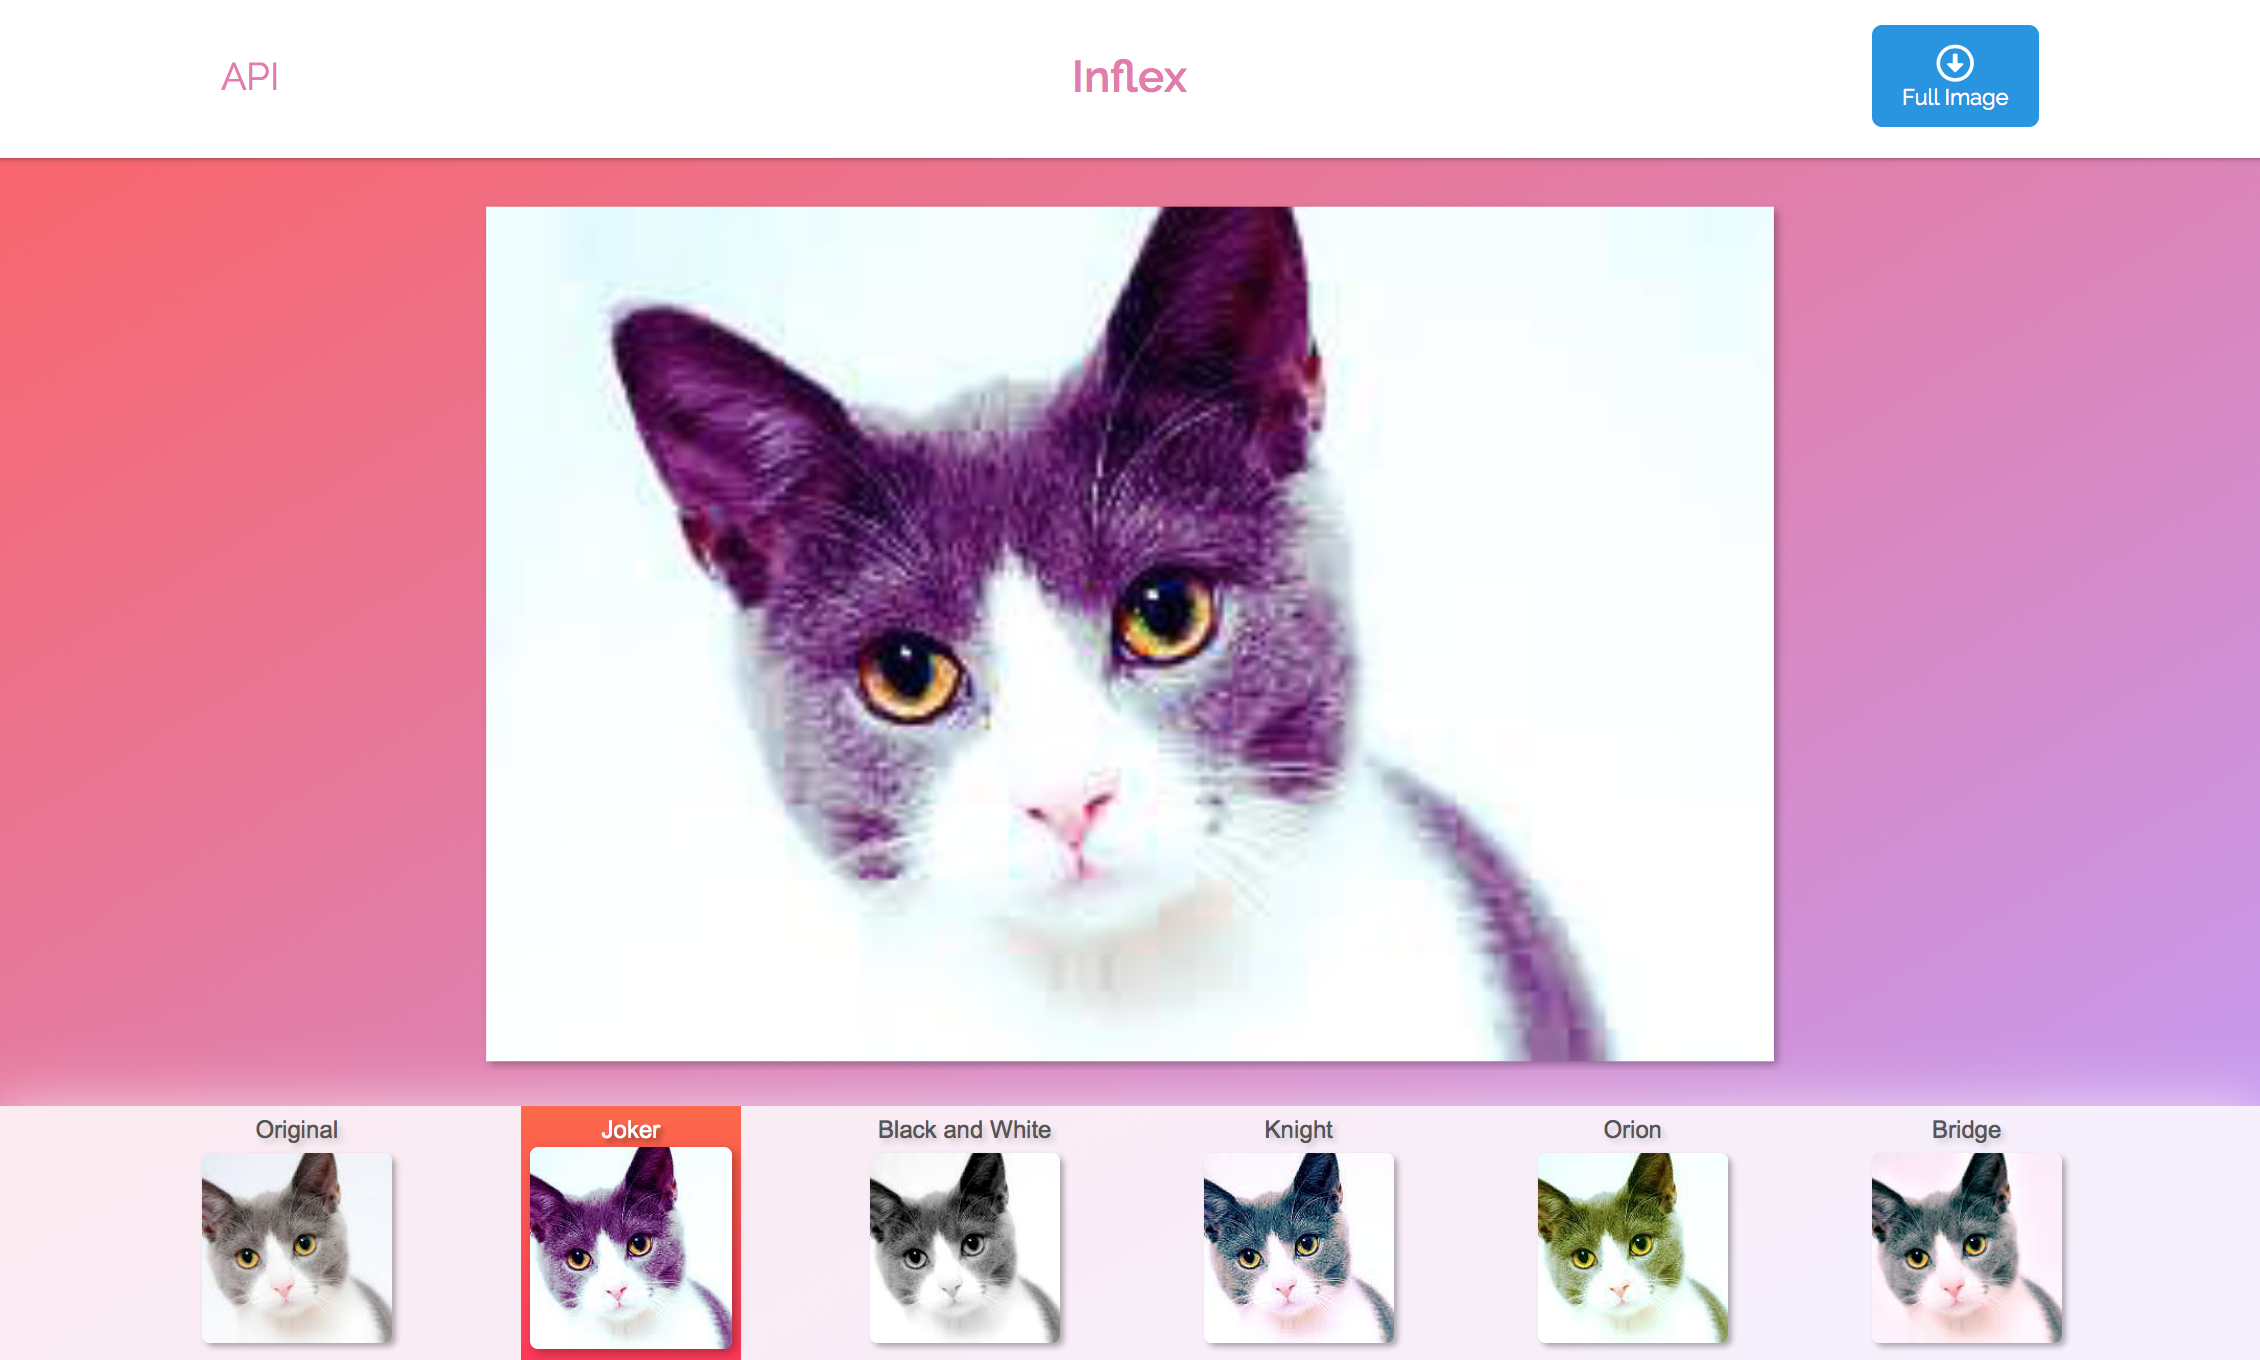
\includegraphics[width=0.7\linewidth]{front-end-main}
      \caption{The filter selection page of the front-end web app}
      \label{fig:front-end-main}
    \end{figure}

    The front-end is comprised of two major components which are the upload / image display area, and the filter thumbnail bar across the bottom of the page. A lot of effort was put into making the site being able to scale to different screen sizes, which turned out to be more difficult than expected. As seen in figure \ref{fig:front-end-main} the image in the center of the page fills most of the negative space between the header and footer. In order to make the center image scale proportionally some code had to be implemented which calculates the correct ratio for the image size and automatically calculates the next best size as soon as the window is re-sized. The result of re-sizing the window to a size more comparable to a mobile screen can be seen in figure \ref{fig:front-end-mobile}.

    \begin{figure}[h]
      \centering
      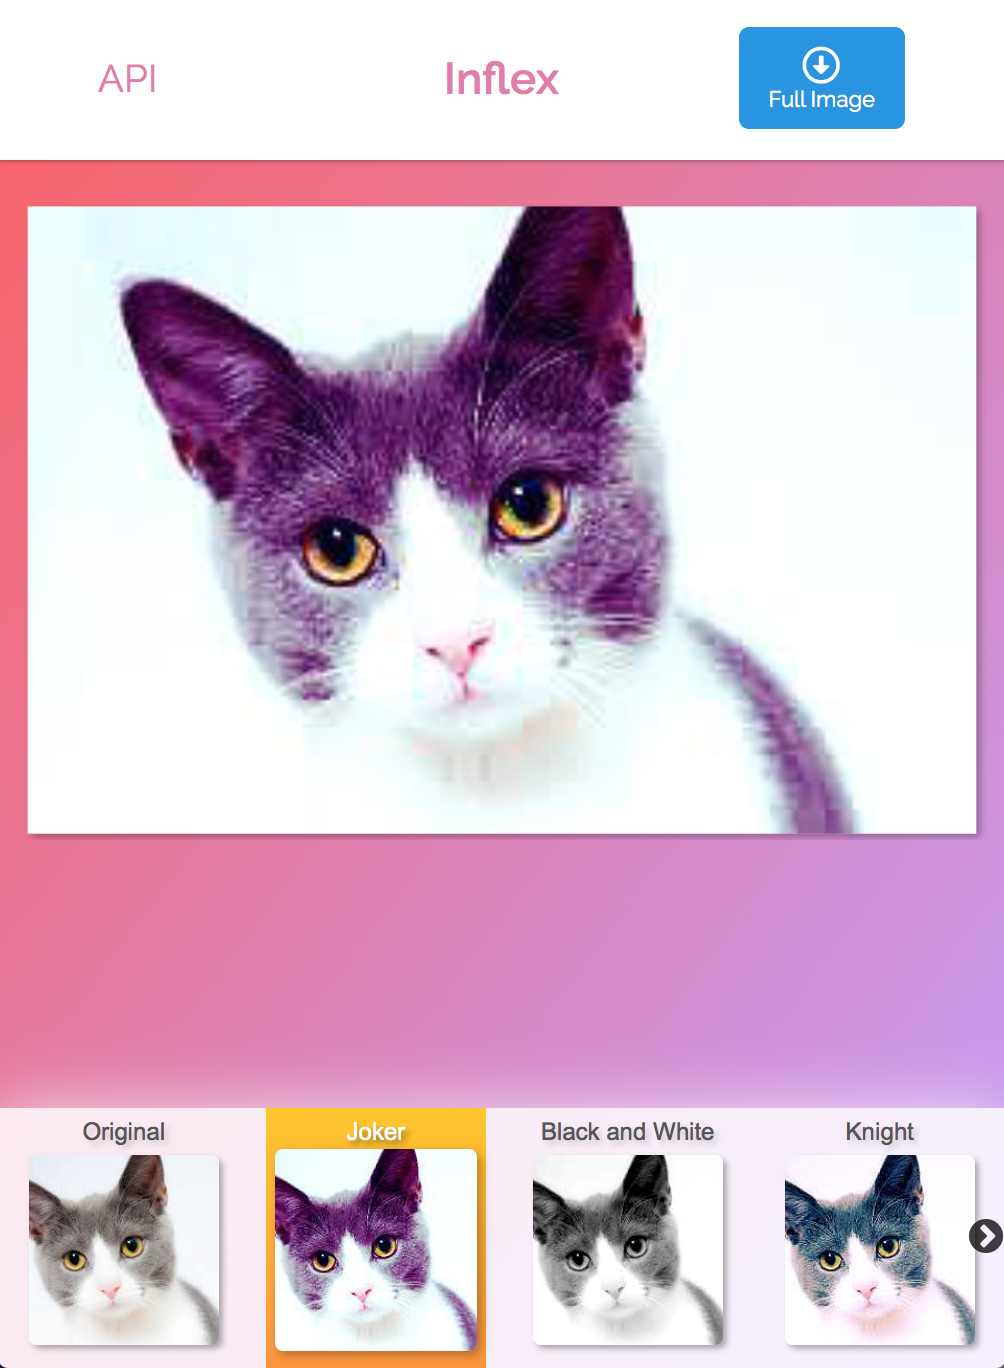
\includegraphics[width=0.5\linewidth]{front-end-mobile}
      \caption{The filter selection page - scaled to a mobile screen size}
      \label{fig:front-end-mobile}
    \end{figure}

    A library called React Slick (\url{https://react-slick.neostack.com}) was used to power animations between different images on the front-end filter selection page. The library has many features built-in which were very useful such as being able to control the state of one image carousel using another - in this case using the thumbnail bar to control the current image in the central area. Both areas are also touch-optimised so on a mobile device it would be possible to quickly swipe between different filters.

    In the top right of figures \ref{fig:front-end-main} \& \ref{fig:front-end-mobile} a blue button can be seen which is the one that a user must click in order for the API to recieve a response that a user has chosen to download an image with a certain filter. Care was taken to make the button stand out from the rest of the page to ensure a user would immediately see it and know what its purpose was. In addition to this, in the bottom of figures \ref{fig:front-end-main} \& \ref{fig:front-end-mobile} one of the filters has a coloured background which is there to indicate that this is the recommended filter. Also when the user uploads their photo and the filters appear on screen, the recommended filter is automatically shown as the central image.

    \newpage

  \section{Deployment}
    The final step for implementing the product proposed in this report is to deploy it to an external server and connect it to a public domain name. The deployment will be carried out in three different sections, which are the API, the front-end and the MongoDB database.

    \subsection{API}
      In the prototype stages of implementing the API in Python, temporary deployments were run in order to test whether an application developed locally would run as planned on a remote server. This ended up causing a lot of frustration but was also very helpful as it outlined the steps which had to be taken and the configuration which had to be used in the final deployment to ensure it ran successfully. One of the problems was that the application would not start up properly when deployed on a server running Python version 3.6. In response to this a test deployment was tried using Python version 3.4 and it successfully ran the application, and since then development and every deployment has been done using Python 3.4 as the language version.

      \begin{figure}[h]
        \centering
        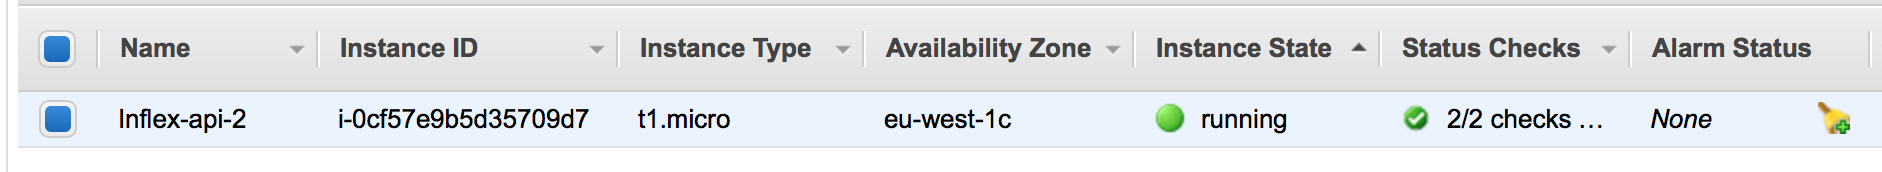
\includegraphics[width=\linewidth]{ec2-info}
        \caption{API Deployment - AWS EC2 instance status}
        \label{fig:ec2-info}
      \end{figure}

      The deployments on AWS were done using the Elastic Beanstalk product which allows for relatively easy set-up. The specific server type which the application is deployed to is a \texttt{t1.micro} server running Python 3.4 on 64bit Amazon Linux version 2.6.4. The server information and running status can be seen in figure \ref{fig:ec2-info} from the AWS EC2 Dashboard page.

      \begin{figure}[h]
        \centering
        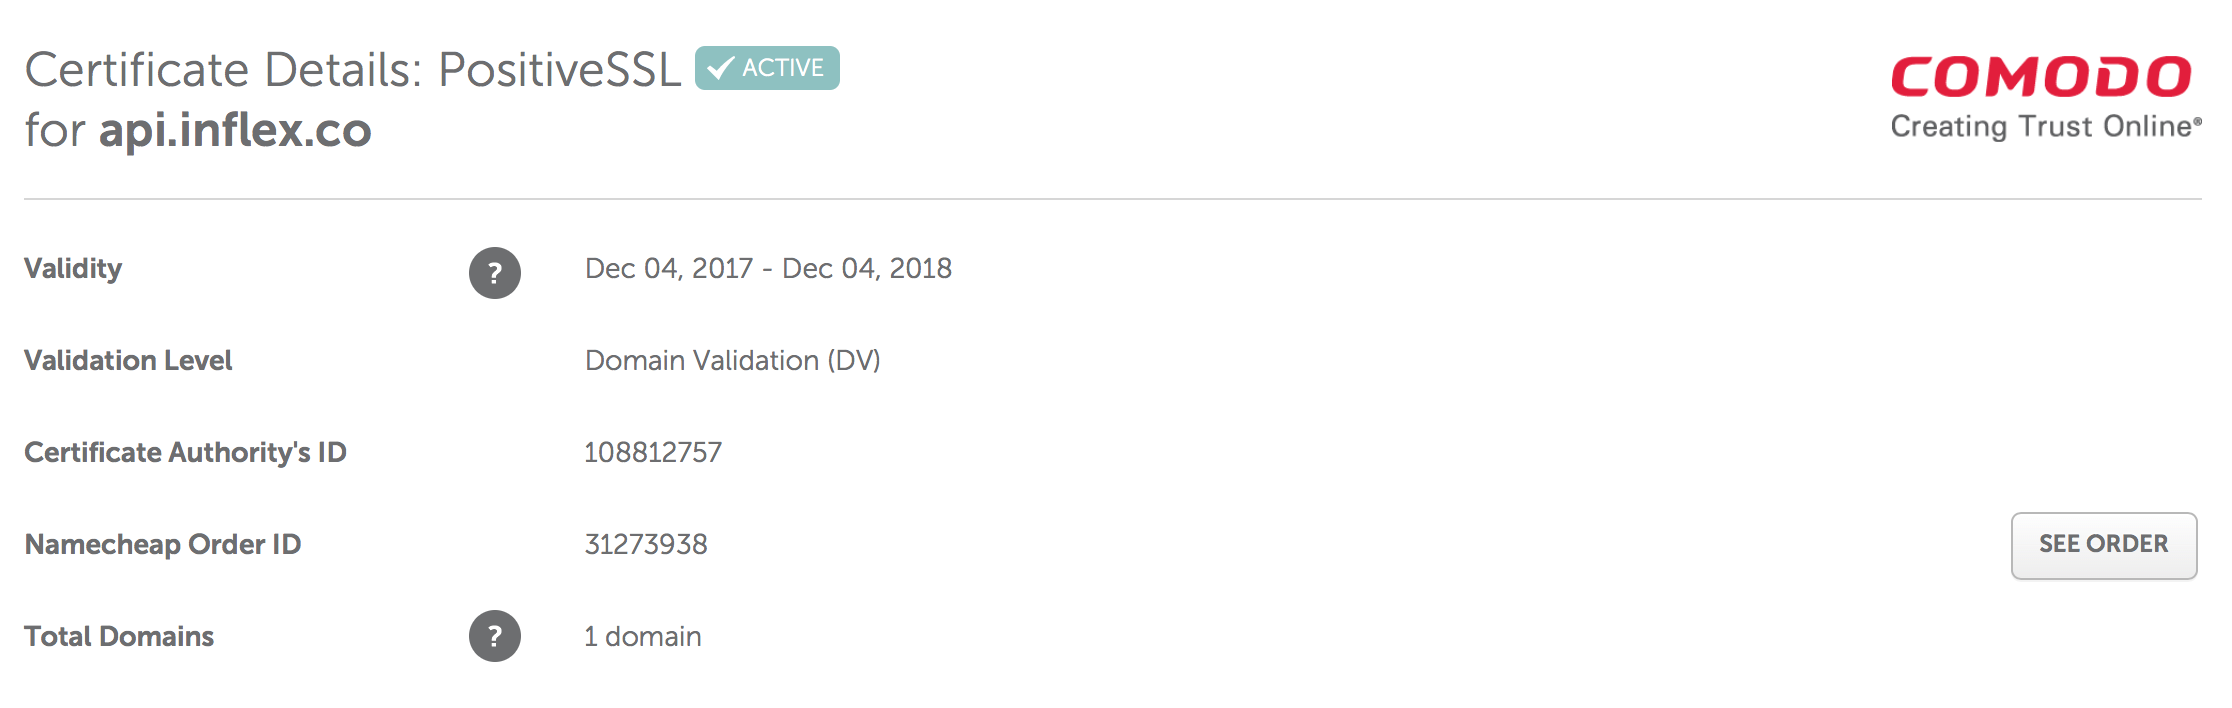
\includegraphics[width=\linewidth]{api-ssl-cert}
        \caption{API Security - Domain SSL certificate information}
        \label{fig:api-ssl-cert}
      \end{figure}

      In order to have an API which could be considered as secure, an important way of achieving this would be to have the service running securely over HTTPS. In order to achieve this an SSL certificate was purchased from the domain provider NameCheap (\url{https://www.namecheap.com}). The certificate provided was then uploaded to the AWS application instance in order for it to start serving traffic over HTTPS. Details about the certificate are shown in figure \ref{fig:api-ssl-cert} and evidence of connecting using this secure protocol is shown in figure \ref{fig:api-ssl-connection}.

      \begin{figure}[h]
        \centering
        
\includegraphics[width=0.3\linewidth]{api-ssl-connection}
        \caption{API Security - Secure connection to API}
        \label{fig:api-ssl-connection}
      \end{figure}

    \subsection{Front-end}
      Deploying the front-end was comparatively simple after deploying the API. The React code can be built using the ‘\texttt{react-scripts build}’ command, which creates a set of files which can be uploaded to a static file hosting server such as AWS S3. Using S3, it is possible to configure the static host to serve the files like a web host and all that needs to be done after that is to point the domain at the static host. As the React code is all based in JavaScript, the resulting front-end is processed entirely on the client therefore a dedicated web service is not required for hosting it.

      Unfortunately, an HTTPS configuration was not achieved on the front-end deployment. However, this is not a huge problem due to the fact that all front-end HTTP calls are made on the client through AJAX, and every call to the API is done over HTTPS as shown in the previous section. This means that any file uploaded to the server is still protected however when downloading the static JavaScript files for the front-end the connection is not secure.

    \subsection{Database}
      Throughout most of the development stages of the application, a local instance of MongoDB was run for testing the application's interactions to the database. Once it was time to deploy a database to an external server an initial effort was made over a week or so to manually set up an instance of MongoDB on an AWS server. Unfortunately the time spent on this ended up being wasted as after many attempts it was still not possible to connect to the MongoDB instance from the API server. After this, it was discovered that MongoDB themselves offer a service called MongoDB Atlas (\url{https://www.mongodb.com/cloud/atlas}) which provides a free instance of cloud-hosted MongoDB (coincidentally hosted on AWS).

      \begin{figure}[h]
        \centering
        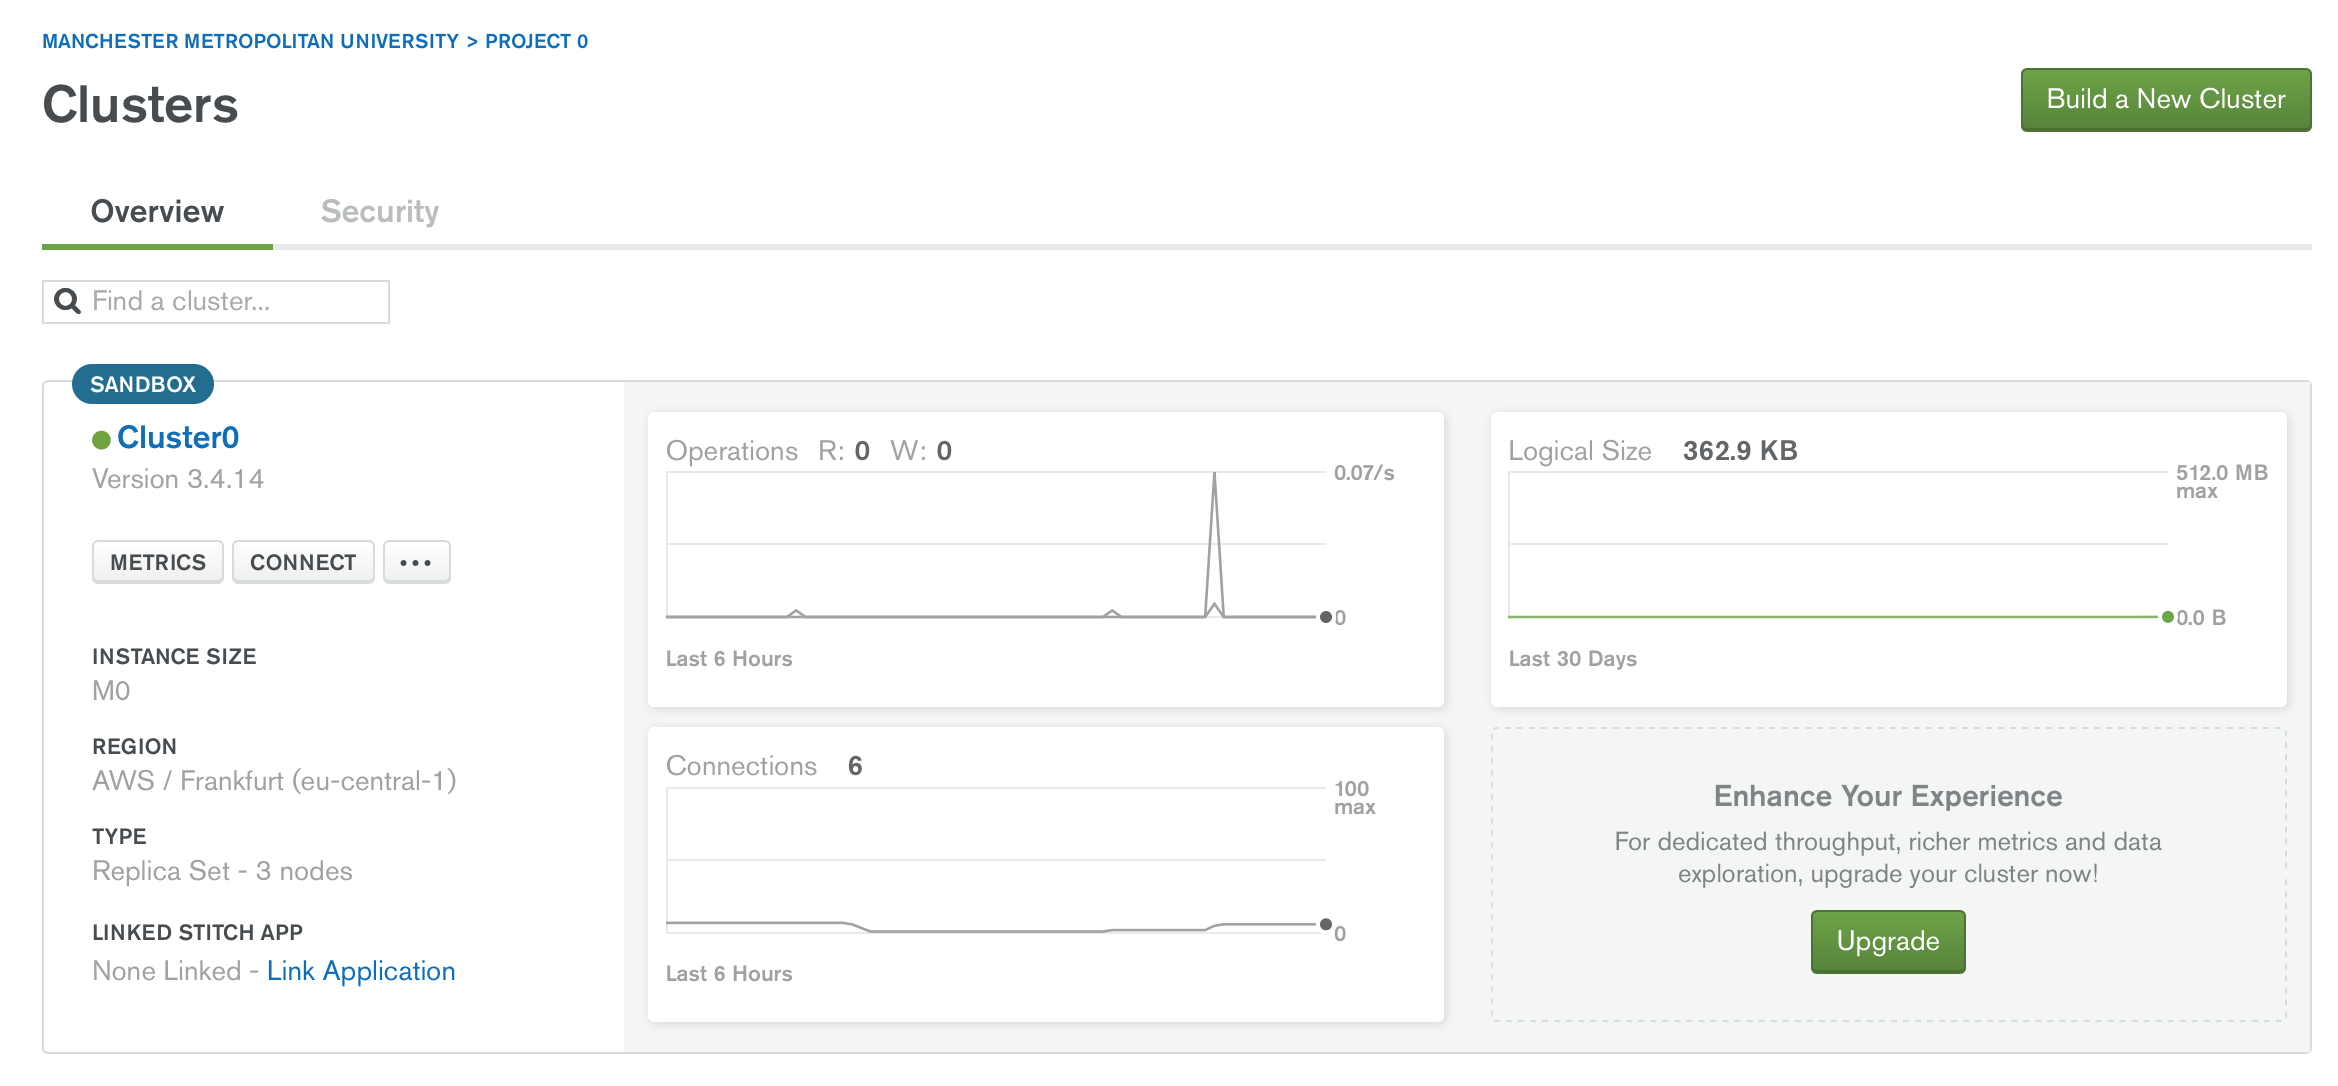
\includegraphics[width=0.8\linewidth]{mongodb-atlas-dashboard}
        \caption{MongoDB Atlas - Deployed cluster dashboard}
        \label{fig:mongodb-atlas-dashboard}
      \end{figure}

      The instance provided by MongoDB Atlas includes a primary server and two replica servers which handle back-ups of data. The dashboard information about the deployed instance used in the application is shown in figure \ref{fig:mongodb-atlas-dashboard}. Once the database service was up and running it was then trivial to change the connection details in the API code to then point at the new service instead of the local service. No further set up was needed to start using the service due to the fact that MongoDB has no constraints on what document structures can be stored on the database. If for example an SQL server was used it would have required runnning lots of SQL scripts to make sure the server was configured correctly before any data could be inputted into it.

\chapter{Evaluation}
  Within this report there were multiple aims which were set out to be achieved. These aims covered a variety of subjects such as computer vision for image analysis and following best practices for developing an API and Web App. The main of these requirements were developing the API, developing the Web front-end, developing a system for filtering images, and most importantly developing a recommender system for those filters. The system proposed and implemented in chapter \ref{cha:implement} meets most of these goals well, and the evaluation of the product will consist of how well the original objectives set out in section \ref{sec:objectives} were met. The objectives and their evaluations are set out below.

  \newpage
  \subsubsection{Objective \ref{obj1} - Implement a simple online web application for filtering images using a framework or library designed for front-end development across multiple platforms.}
    The front-end propsosed in this report is very effective in its use as an interface on top of the API. It is very lightweight and simple however it is also very functional and robust. The use of React really helped to streamline the development as it meant the structure in the code of the front-end was already much easier to work with. The component structure allows for very easy management of application flow, with variables and callback functions being passed to child components the application is easily able to deal with calling an external API and passing that information to components which automatically update upon recieving that information. However, the requirement for the web app working across multiple platforms was not met. During development the front-end was run purely on a few different desktop browsers such as Safari and Chrome which worked perfectly, however after finally deploying it to a public URL and accessing it from a mobile device it was found that no response came back to the device once an image was uploaded for filtering. Due to the nature of mobile devices there was no easy way to troubleshoot what was going on, where on a desktop device this could easily be done by debugging it in an IDE. Finally, there was not enough time after deploying the application to do an investigation into this issue therefore it can only be viewed as a partial failure to meet one of the objectives.

  \subsubsection{Objective \ref{obj2} - Implement a back-end application which is able to process images including applying filters and creating thumbnails.}
    The python back-end proposed in this report is highly capable of processing images due to the libraries available and its ability to connect easily to the API code. The libraries NumPy and Pillow were both instrumental to the success of image processing, however there was a decent learning curve to both of these along with python itself. This slightly limited how much processing was able to be done on the images as much more time had to be spent researching what libraries are available and what the best practices are for processing images in python. The code design proposed helped very much in how the filters connected to the API, as each filter was a sub-class of a base filter the filters could easily be run by looping through the ‘\texttt{\_\_subclasses\_\_()}’ method on the base class, passing in the ‘\texttt{Filterable}’ object each time. The ‘\texttt{Filterable}’ class also allowed the images to be quickly converted from Pillow types to NumPy types, and also to resize the image into different sizes such as thumbnail and preview sizes.

  \subsubsection{Objective \ref{obj3} - Research various recommender systems to determine the common technologies/solutions for solving the problem of recommendations.}
    In section \ref{sec:lit-recc} various examples of recommender systems were found and a general concensus was discovered that machine learning tools are a very useful tool in recommender systems. While there was not a single blanket solution, and the solutions available are often still not very effective - facing issues such as the cold-start problem which is still a popular research topic. Deep learning was discovered to be a very common tool in industry however this was not feasible due to performance constraints and that they did not seem to be fully applicable to the problem of recommending filters.

  \subsubsection{Objective \ref{obj4} - Implement a recommender system which is able to suggest photo filters to users based on image content.}
    Within this objective the strict definition was met, as a recommender system was built which is able to recommend filters based on image content. However, the accuracy of the AI system which was implemented was not very high, and often came up with highly inconsistent values when producing classification accuracy reports. When using a trained model with a higher trained accuracy of around 35\% on average per class, the model did however seem to have some predictability in how it would recommend filters such as when the photo included one or more faces. The low accuracy would seem to suggest that the method for training the model was not ideal in that users may have had differing tastes for which filters to apply. Furthermore the recommender would occasionally suggest different recommendations when the same photograph was uploaded twice. This is likely a combination of the K-Means analysis producing slightly different results each time and the classifiers not having a strong enough trained model.

  \subsubsection{Objective \ref{obj5} - Implement a RESTful API which exposes both the recommender system and the filtering system to the front-end web app and allows developers to connect them into their own applications.}
    This objective was met easily with the python back-end using the Flask library. This library included helper methods for handling RESTful API's and allowed for doing things such as responding with an ‘\texttt{HTTP 201 CREATED}’ response when a resource was uploaded to the site via an ‘\texttt{HTTP POST}’ request. The URI structure was also within REST constraints, with images being uploaded to the ‘\texttt{/images/}’ URL via an ‘\texttt{HTTP POST}’ request, then being accesed using an ‘\texttt{HTTP GET}’ request from that URL such as\\ ‘\texttt{/images/98119-black\_and\_white.jpg}’. The URI structure was relatively simple due to the simplicity of the request being made therefore it was easier to develop. The responses from the API were also very easy to output as JSON due to python's ability to define a ‘\texttt{dict}’ object using a very similar syntax to JSON, directly in the code. This ‘\texttt{dict}’ object could then easily be translated into an HTTP response using Flask's ‘\texttt{jsonify()}’ method. The API was then easily connected to the front-end and using React which is based in JavaScript made handling JSON responses that much easier, due to JavaScript's high integration with JSON (which makes sense as JSON stands for JavaScript Object Notation...).

\chapter{Conclusion}
  This report has outlined a system which can be used to filter photographs by accessing a REST API, or by connecting to an accompanying web app using a desktop web browser. The API and web app are able to give a recommendation of which filter should be chosen based on the content of the image, however this recommendation was not proven to be very accurate. The code solution is simple and includes many carefully chosen libraries to handle difficult tasks, rather than implementing them manually which creates unnecessary work and introduces too much complexity into the product. Due to time constraints some issues were left unsolved such as not having HTTPS on the front-end server and the front-end not working on mobile devices.

  \newpage
  \section{Further work}
    If offered more time to extend the functionality of the product, initially the existing problems mentioned in the preceeding paragraph could be addressed. Further to solving those issues, as a result of the low accuracy from the recommendation algorithm a more advanced recommender algorithm could be implemented. This could include developing a user system which is able to track individual user history for applying photo filters and have that data be used to provide more personalised recommendations for users. Additionally, background processing could be introduced where uploaded images are not analysed and filtered synchronously but are done at the same time in order to reduce response times.

  \section{Author reflection}
    When starting this project I set out a personal goal to learn a few different technologies such as Python, React, and AWS. I do feel like I was able to do this and also create a product which serves its purpose relatively well. However, I think the biggest hindrance throughout the project was that every time I started work on a different part of the product implementation I would have to start from absolute scratch, spending more time learning the basics than implementing desired features. This lead to some gaps in quality of code design, and features which never made it into the final product.

    Overall, I have enjoyed the process of completing this project and it feels like the true summation of all the work I have put in over my whole university career. I hope to utilise lessons learned from this project throughout my later life in both programming and real life.

\newpage
\singlespacing

\bibliographystyle{agsm}
\bibliography{report}

\end{document}
